\documentclass[../main.tex]{subfiles}

\begin{document}

The system was fully tested only on linux environment, for which the following instructions will be valid, though it should run on all major platforms with proper adjustments. To evaluate all components of this prototype, at least these software packages must be installed and working on the system in use:

\begin{itemize}
	\item Node JS (11.6.0)
	\item npm (6.5.0)
	\item Flutter (1.0.0 - rev. 5391447fae)
	\item Dart (2.1.0)
	\item JDK/OpenJDK 8
	\item Android Studio or Intellij Idea - for the wearable application
\end{itemize}

In parenheses is indicated the version used in development. Following are the steps to launch the various components:

\subsection{Backend server}

\begin{itemize}
	\item Eventually import the project ITD/TrackMeServer in Android Studio / Intellij Idea (not required).
	\item Navigate to ITD/TrackMeServer and run "npm install" to download the required dependencies (defined in package.json).
	\item Edit the common/config.json file with address and port on which each component should listen for incoming connections.
	\item Edit the common/config.json file setting to "true" the postgres.useHeroku variable to use an already set up DBMS. It is though advised to use a local DBMS connection (PostgresQL) if possible, since it allows to browse the data in the database. In this case, set the useHeroku variable to "false" and properly set the other three variables.
	\item Run the components by executing \newline "node DatabaseServer/DatabaseServer.js \& \newline node ApplicationServerMobileClient/ApplicationServerMobileClient.js \& \newline node ApplicationServerData4Help/ApplicationServerData4Help.js \& \newline node WebServer/WebServer.js \&" \newline or by launching them from the IDE.
\end{itemize}

Note that the working directory for the processes must be ITD/TrackMeServer, otherwise some necessary files won't be found. Also, each module can be launched on a different directory, or a different host, as long as the "common" and "node\textunderscore modules" directories are present along the component's one.

Also, every variable defined in config.json can be overridden with environment variables. The structure of such variables is equal to the ones in the configuration file, with the following differences: all character are uppercase, and to address a sub-variable, use the underscore. For example, to temporarily use the heroku DBMS, one could launch the DatabaseServer like this:\newline
POSTGRES\textunderscore USEHEROKU=true node DatabaseServer/DatabaseServer.js

\subsubsection{Support files for evaluation}

Inside the "support" directory there are some files useful for evaluating the project, as stated in chapter 4. To launch the python scripts, just run "python3 \textit{path-to-py-file}". Note that they also need the common/config.json file to be in the working directory.

A Postman configuration, that was also used for testing, is also supplied. To import it, just launch Postman, then click import and open postman.json file. The following functions are defined: \newline

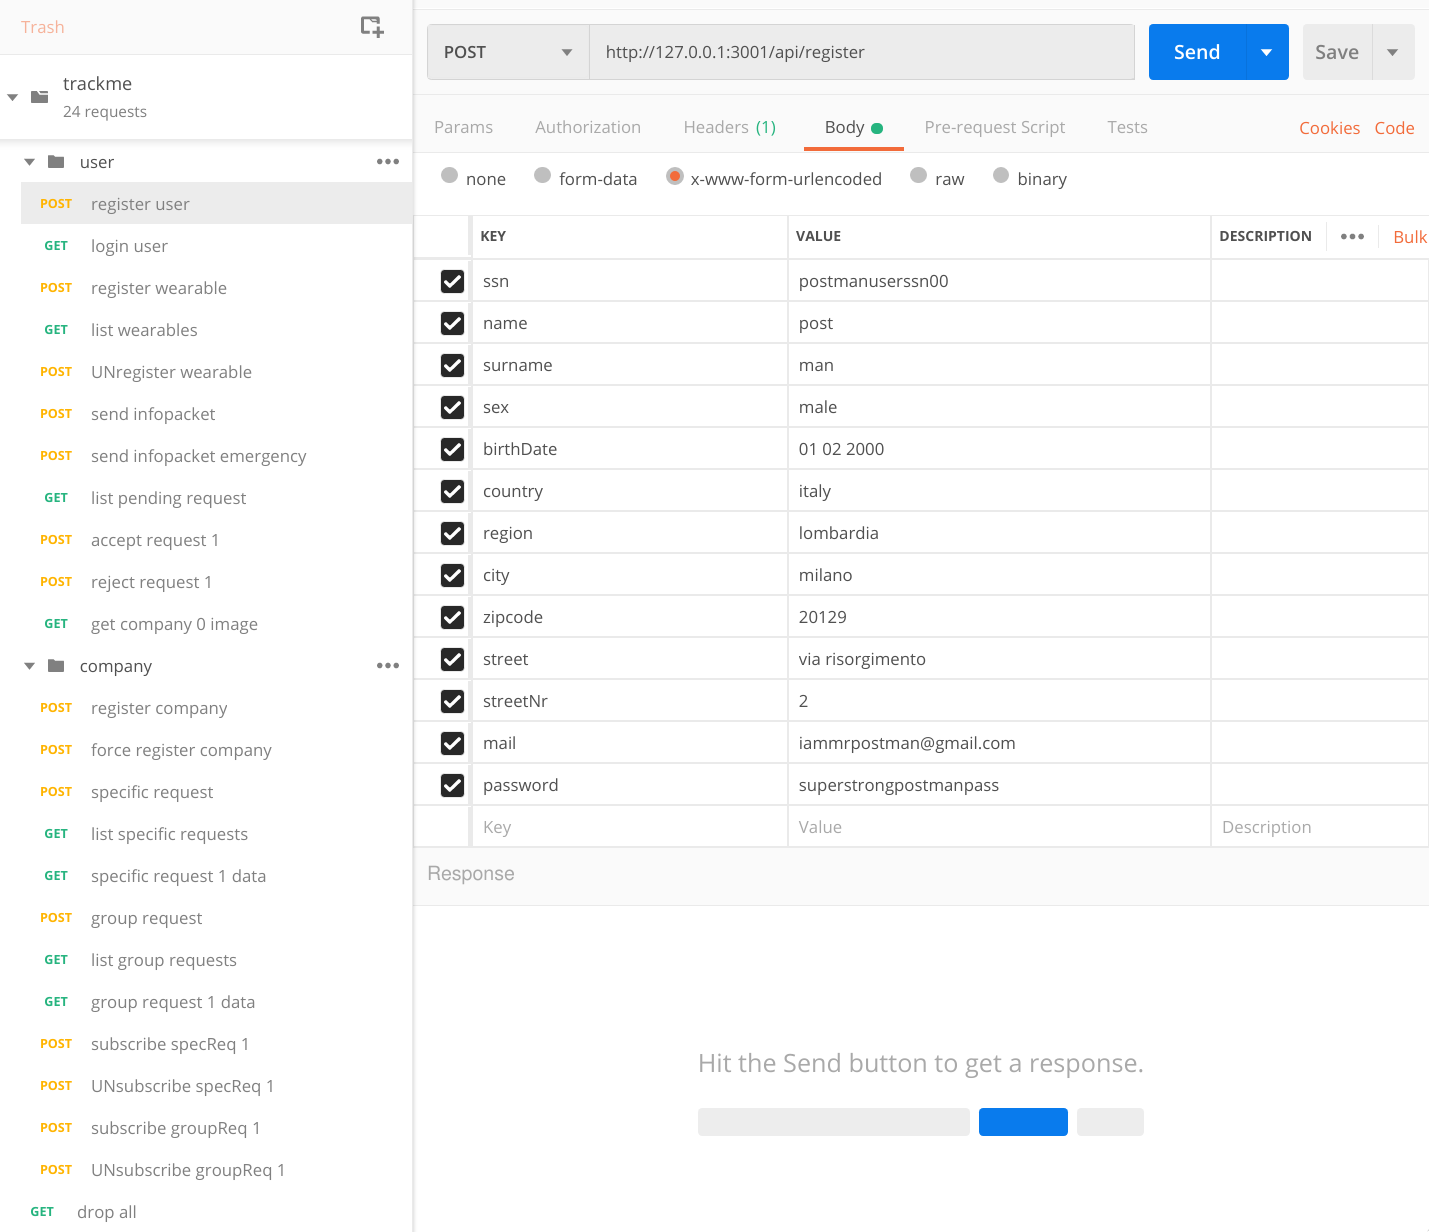
\includegraphics[width = \linewidth ]{images/postman_screen.png}

\end{document}
